%!TEX root = ../dissertation.tex

\chapter{Environment Overview}
\label{sec:network_overview}
There are many applicability domains and different methods for creating \gls{IoT} networks. 
Some provide direct connectivity of nodes to the Internet while others provide a common gateway for interfacing with external networks. 
In our work, we focus on scenarios where network nodes are not directly connected to the Internet and require additional network components for proper communication as depicted in Figure \ref{fig:net_overview}.

\begin{figure}[h]
  \centering
  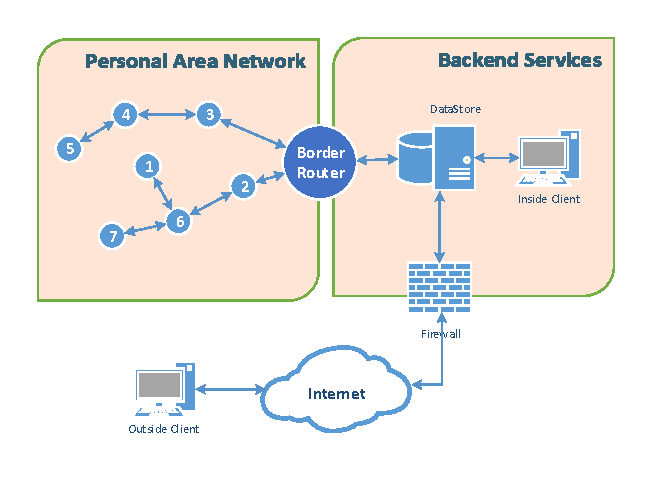
\includegraphics[width=0.8\linewidth]{figures/Network_Overview.pdf}
  \caption{IoT Network Overview.}
  \label{fig:net_overview}
\end{figure}

In this type of architectures, the sensing or actuating nodes belong to a very constrained network with specific protocols and header compression mechanisms, requiring an interface device -- the border router -- in order to communicate with external networks.
After reaching the external network, incoming messages are processed to convert sensor data into useful information which is then stored or used to trigger events. 
This information can then be accessed by users either on the same network or by making requests through the Internet. 

This type of deployment could be used, for example, in a home intrusion system or in a factory monitoring system. 
In the home intrusion system scenario, the network nodes would create a sensor network that propagates events in the case of an intrusion and the additional infrastructure would be in charge of receiving these events and notifying the police authorities. 
In the factory monitoring system scenario, the network nodes would create a sensor network that would be permanently reporting up-to-date readings of machinery control values like: temperature, pressure and power; 
and the additional infrastructure would in charge of supplying this information to a dashboard for the factory workers. 
If an attacker could disable these systems, he could then 
%rob the house or 
cause an emergency shut-down of the factory machinery due to lack of control over the working conditions. 
These are real concerns backed by a range of attacks that focuses on disabling \gls{IoT} networks by placing the nodes offline. These attacks are presented in the following Section.